% ==============================================================================
% VientoVis — Entrega 2: el proceso de diseño (la visualización salta al mundo físico)
% IIC2026 · Proyecto de Visualización de Información · 2026-2
%
% Estructura según el enunciado (https://infovis.alessiobellino.com/e2):
%   §11 Plantilla del documento (orden obligatorio):
%       Portada → Contexto general → V1 → R1 → V2 → R2 → V3 → R3 → V4
%       → El feedback al otro grupo → Evaluación con usuarios (una subsección por ronda)
%   §10 Rúbrica: Proceso iterativo 25 % · Rationale 25 % · Revisiones 15 %
%       · Feedback al otro grupo 10 % · Prototipo final 15 % · Evaluación con usuarios 10 %
%   §12 Checklist previo a la entrega (anexo al final)
%
% Convenciones de este archivo:
%   \pendiente{...}  → texto en rojo que AÚN FALTA completar. Antes de entregar,
%                      buscar "\pendiente" y que no quede ninguno.
%   % FOTO: / % VIDEO: → lugares donde van fotografías y links a videos
%                      (comentados hasta tener el material).
%   Los límites de líneas del enunciado están anotados en cada bloque (máx. N líneas).
%
% Compilar desde documento/entrega2/:  pdflatex entrega2.tex  (dos pasadas)
% ==============================================================================
\documentclass[11pt,a4paper]{article}

\usepackage[utf8]{inputenc}
\usepackage[spanish,es-tabla]{babel}
\usepackage[margin=2.0cm,top=2.2cm,bottom=2.2cm]{geometry}
\usepackage{lmodern}
\usepackage{amssymb}
\usepackage{xcolor}
\usepackage{graphicx}
\usepackage{caption}
\usepackage{booktabs}
\usepackage{tabularx}
\usepackage{enumitem}
\usepackage{titlesec}
\usepackage{fancyhdr}
\usepackage{microtype}
\usepackage[many]{tcolorbox}
\usepackage{hyperref}

% Imágenes: primero las de esta entrega, luego las compartidas con la Entrega 1
\graphicspath{{figuras/}{../figuras/}}

% Paleta de colores acorde a la identidad visual de VientoVis (igual que Entrega 1)
\definecolor{ink}{HTML}{1A1A1A}
\definecolor{brick}{HTML}{C8442A}
\definecolor{wood}{HTML}{8C532B}
\definecolor{ochre}{HTML}{C98A2C}
\definecolor{paper}{HTML}{F9F6F0}
\definecolor{softgray}{HTML}{E8E4DC}
\definecolor{darkgray}{HTML}{4A4A4A}

% Marcador de contenido por completar (visible en el PDF para que no se escape)
\newcommand{\pendiente}[1]{{\color{red}\textbf{[PENDIENTE:} #1\textbf{]}}}
% Lectura dudosa de un manuscrito: se muestra el texto seguido de [?] en rojo
\newcommand{\dudoso}[1]{#1\,{\color{red}\textbf{[?]}}}

% Configuración de hipervínculos
\hypersetup{
	colorlinks=true,
	linkcolor=brick,
	filecolor=brick,
	urlcolor=brick,
	citecolor=brick,
	pdftitle={Entrega 2 - Proyecto de Visualización de Información (VientoVis)},
	pdfauthor={Esperanza Oliva, Florencia Taís Rojas, Esteban Arias, Vicente Pardo}
}

% Encabezados y pies de página
\pagestyle{fancy}
\fancyhf{}
\fancyhead[L]{\small\color{darkgray}\textbf{IIC2026} · Proyecto de Visualización de Información}
\fancyhead[R]{\small\color{darkgray}\textbf{VientoVis} — Entrega 2}
\fancyfoot[C]{\thepage}
\renewcommand{\headrulewidth}{0.4pt}
\renewcommand{\footrulewidth}{0.4pt}

% Formato de títulos
\titleformat{\section}{\Large\bfseries\color{ink}}{\thesection.}{0.6em}{}[\vspace{-0.2em}\titlerule]
\titleformat{\subsection}{\large\bfseries\color{brick}}{\thesubsection}{0.6em}{}
\titleformat{\subsubsection}{\normalsize\bfseries\color{wood}}{\thesubsubsection}{0.6em}{}

% Cajas de contenido estilizadas y breakables
\newtcolorbox{metabox}{
	breakable,
	colback=paper,
	colframe=ink,
	boxrule=1pt,
	arc=4pt,
	left=12pt, right=12pt, top=10pt, bottom=10pt
}

\newtcolorbox{versionbox}[2]{
	breakable,
	colback=paper,
	colframe=brick,
	fonttitle=\bfseries\color{white},
	title={\large #1\par\vspace{2pt}{\normalsize\mdseries #2}},
	arc=4pt,
	boxrule=1pt,
	left=10pt, right=10pt, top=8pt, bottom=8pt,
	coltitle=white
}

\newtcolorbox{revisionbox}[2]{
	breakable,
	colback=paper,
	colframe=wood,
	fonttitle=\bfseries\color{white},
	title={\large #1 \hfill \normalsize #2},
	arc=4pt,
	boxrule=1pt,
	left=10pt, right=10pt, top=8pt, bottom=8pt,
	coltitle=white
}

\setlist[itemize]{noitemsep, topsep=2pt, leftmargin=1.4em}
\setlist[enumerate]{noitemsep, topsep=2pt, leftmargin=1.4em}

\begin{document}

	% ==============================================================================
	% 1. PORTADA: número de grupo, integrantes y los tres enlaces (§11.1)
	% ==============================================================================
	\begin{center}
		{\scshape\Large Pontificia Universidad Católica de Chile}\\[0.2cm]
		{\large Escuela de Ingeniería · Departamento de Ciencia de la Computación}\\[0.15cm]
		{\large IIC2026 — Visualización de Información · Semestre 2026-2}\\[0.8cm]

		\begin{tcolorbox}[colback=ink, colframe=ink, arc=6pt, halign=center, left=15pt, right=15pt, top=14pt, bottom=14pt]
			{\color{white}\Huge \textbf{VientoVis}}\\[0.25cm]
			{\color{ochre}\LARGE \textit{Los 10 huracanes con más impacto según su mortalidad y pérdida económica}}\\[0.2cm]
			{\color{softgray}\large La visualización salta al mundo físico: proceso de diseño de una experiencia físico-digital y sonora}
		\end{tcolorbox}
		\vspace{0.4cm}

		{\large \textbf{Documento Oficial de Entrega 2}}\\[0.4cm]

		\begin{metabox}
			\textbf{Grupo:} 32\\[0.15cm]
			\textbf{Integrantes:}
			\begin{itemize}[leftmargin=1.2em]
				\item Esperanza Oliva
				\item Florencia Taís Rojas
				\item Esteban Arias
				\item Vicente Pardo
			\end{itemize}
			\vspace{0.25cm}
			\textbf{Enlaces obligatorios de la entrega:}
			\begin{itemize}[leftmargin=1.2em]
				\item \textbf{Parte digital (GitHub Pages):} \href{https://vpardos.github.io/vientovis/}{https://vpardos.github.io/vientovis/}
				\item \textbf{Repositorio (GitHub):} \href{https://github.com/vpardos/vientovis}{https://github.com/vpardos/vientovis}
				% VIDEO: video demostrativo público (YouTube u otro) del prototipo final,
				%        mostrando la interacción física y sonora COMPLETA. Reemplazar la línea siguiente:
				% \item \textbf{Video demostrativo del prototipo final (V4):} \href{https://youtu.be/XXXXXXXXXXX}{https://youtu.be/XXXXXXXXXXX}
				\item \textbf{Video demostrativo del prototipo final (V4):} \pendiente{link al video}
			\end{itemize}
		\end{metabox}
	\end{center}

	\vspace{0.2cm}

	% ==============================================================================
	% 2. CONTEXTO GENERAL (§7): va una sola vez en el documento
	% ==============================================================================
	\section{Contexto General}

	\subsection{Propósito de la Fisicalización}
	% máx. 10 líneas. Por qué la experiencia física hace evidente algo que la pantalla
	% sola no lograba: qué dato se lleva al mundo físico y por qué ese.
	La fisicalización busca que la experiencia sea más interactiva: en lugar de simular digitalmente el efecto de un huracán, el viento del huracán que se está reproduciendo sale de un ventilador real y actúa sobre una maqueta. Así se ve, y se siente, cómo se mueven el tejado de la casa y la palmera a medida que cambia la intensidad, lo que hace tangible el impacto que en la pantalla solo se lee como cifras y gráficos.

	\subsection{Procesamiento de los Datos}
	% máx. 8 líneas. Si los datos se procesaron o ajustaron para la interacción tangible
	% o la fisicalización, y cómo. Mencionar si se mantiene el dataset de la Entrega 1.
	Se mantiene el mismo dataset de la Entrega 1, sin cambios; lo que se ajusta es cómo los datos llegan a la maqueta.
	\begin{itemize}
		\item \textbf{Viento $\rightarrow$ ventilador:} la velocidad del viento del punto activo se traduce en potencia del ventilador con una curva anclada en los umbrales Saffir-Simpson. Parte en 28\,\% (bajo eso un ventilador de 12\,V no gira) y llega a 100\,\% solo en el pico de la serie (Irma, 155\,kt), para que Cat 4 y Cat 5 se distingan.
		\item \textbf{Categoría $\rightarrow$ servo (mueve la casa):} las seis categorías se agrupan en cuatro ángulos (T.T./TD 30°, Cat 1--2 45°, Cat 3--4 60°, Cat 5 75°), enviados solo cuando la categoría cambia.
	\end{itemize}

	\vspace{0.4cm}

	% ==============================================================================
	% 3. V1 — LA IDEA COMPLETA (AUNQUE SIMULADA)
	%    Toda la experiencia de una vez: qué se fisicaliza y por qué, cómo se interactúa,
	%    qué suena y dónde entra la capa digital. Maquetas de cartón / Mago de Oz válidos.
	% ==============================================================================
	\begin{versionbox}{V1 — La Idea Completa (aunque simulada)}{3 de noviembre de 2026 · Sin commit: prototipo local (\texttt{fan.html})}
		\noindent\textbf{Evidencia:} Página de control del ventilador funcionando en el navegador (\textit{Figura~\ref{fig:v1-foto1}}).
		% Fotos del estado físico: OBLIGATORIAS en todas las versiones.
		% Video corto con manipulación y sonido: desde que haya interacción que mostrar.
		% VIDEO: Video de la versión: \href{https://youtu.be/XXXXXXXXXXX}{https://youtu.be/XXXXXXXXXXX}.

		% FOTO: v1_foto1.jpg es la imagen enviada para V1 (con el botón de "play" del video encima).
		%       Reemplazar por el original si se tiene.
		\begin{center}
			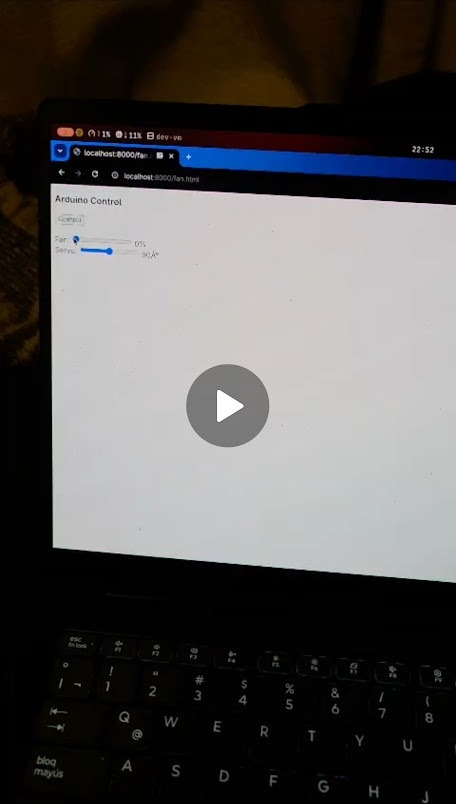
\includegraphics[height=8cm]{v1_foto1.jpg}
			\captionof{figure}{V1: página HTML de control (\texttt{fan.html}, servida en \texttt{localhost}) con los controles deslizantes «Fan» y «Servo».}
			\label{fig:v1-foto1}
		\end{center}

		\vspace{0.15cm}
		\noindent\textbf{Qué cambió (respecto de la Entrega 1):}
		% máx. 8 líneas. Lista concreta.
		\begin{itemize}
			\item Primera versión de una página HTML funcional que controla el ventilador físico.
		\end{itemize}
		\pendiente{completar cambios de V1 (máx. 8 líneas)}

		\vspace{0.15cm}
		\noindent\textbf{Por qué cambió — el rationale:}
		% máx. 12 líneas. Lo que más pesa en la rúbrica (25 %). Anclado en principios del curso,
		% discusiones de revisiones, feedback de usuarios, evidencia del dato o restricciones documentadas.
		\pendiente{rationale de V1 (máx. 12 líneas)}

		\vspace{0.15cm}
		\noindent\textbf{Qué se descartó:}
		% máx. 5 líneas. Alternativas probadas y abandonadas, y por qué.
		\pendiente{descartes de V1 (máx. 5 líneas)}
	\end{versionbox}

	\vspace{0.4cm}

	% ==============================================================================
	% 4. R1 — REVISIÓN CON EL EQUIPO DOCENTE (entre V1 y V2)
	%    Fecha · síntesis breve · decisiones (adoptado / descartado y por qué). Máx. 10 líneas.
	% ==============================================================================
	\begin{revisionbox}{R1 — Revisión con el Equipo Docente}{3 de noviembre de 2026}
		\noindent\textbf{Fecha:} 3 de noviembre de 2026.\\
		\textbf{Síntesis de lo discutido:} No se presentó con la maqueta completa, ya que se nos quedó; la revisión consistió en la presentación formal de la idea. \pendiente{quién revisó y qué se discutió}

		\vspace{0.15cm}
		\noindent\textbf{Decisiones tomadas (adoptado / descartado y por qué):}
		\pendiente{decisiones}
	\end{revisionbox}

	\vspace{0.4cm}

	% ==============================================================================
	% 5. V2 — PRIMERA ITERACIÓN DE DISEÑO (tras R1)
	%    Qué no funcionó en la forma física, la interacción tangible y el sonido.
	% ==============================================================================
	\begin{versionbox}{V2 — Primera Iteración de Diseño}{12 de noviembre de 2026 · Commits \texttt{85024f3}, \texttt{fc84d25}, \texttt{ecad690}, \texttt{0ae2df0}}
		\noindent\textbf{Evidencia:}
		Ventilador funcionando conectado al Arduino (\textit{Figura~\ref{fig:v2-foto1}}).
		% VIDEO: Video de la versión: \href{https://youtu.be/XXXXXXXXXXX}{https://youtu.be/XXXXXXXXXXX}.

		% FOTO: v2_foto1.jpg es la imagen enviada para V2.
		\begin{center}
			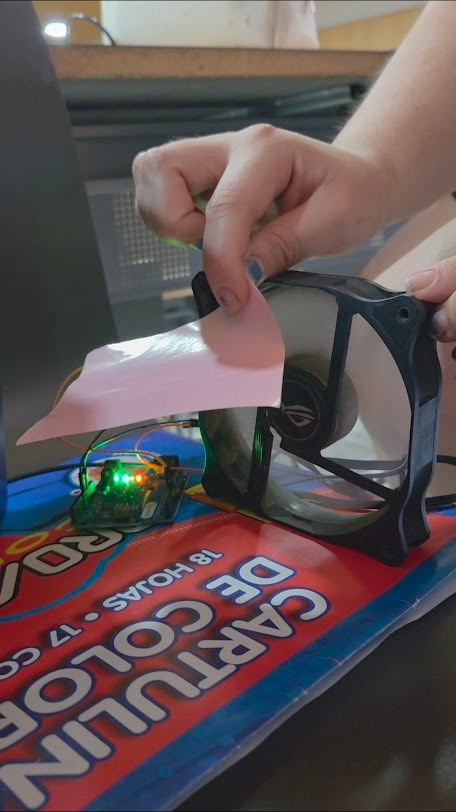
\includegraphics[height=8cm]{v2_foto1.jpg}
			\captionof{figure}{V2: el ventilador, conectado al Arduino, mueve una hoja de papel.}
			\label{fig:v2-foto1}
		\end{center}

		\vspace{0.15cm}
		\noindent\textbf{Qué cambió:}
		% máx. 8 líneas.
		\begin{itemize}
			\item El ventilador funciona sincronizado con la página del proyecto.
			\item Se construye la casa de cartón que recibe el viento del ventilador (en V1 no existía).
		\end{itemize}
		\pendiente{completar cambios de V2 (máx. 8 líneas)}

		\vspace{0.15cm}
		\noindent\textbf{Por qué cambió — el rationale:}
		% máx. 12 líneas.
		\pendiente{rationale de V2 (máx. 12 líneas)}

		\vspace{0.15cm}
		\noindent\textbf{Qué se descartó:}
		% máx. 5 líneas.
		\pendiente{descartes de V2 (máx. 5 líneas)}
	\end{versionbox}

	\vspace{0.4cm}

	% ==============================================================================
	% 6. R2 — REVISIÓN ENTRE PARES (entre V2 y V3). Máx. 10 líneas.
	% ==============================================================================
	\begin{revisionbox}{R2 — Revisión entre Pares}{12 de noviembre de 2026}
		\noindent\textbf{Fecha:} 12 de noviembre de 2026.\\
		\textbf{Síntesis de lo discutido:} Al usarlo, el grupo evaluador entendió la intensidad del huracán y su impacto en las estructuras (ventilador y casa de cartón). El impacto se aprende de forma cualitativa, pero se pierde cuantitatividad: con el ventilador cuesta notar diferencias sutiles de intensidad. Pidieron conservar el ventilador y la casa, por ser intuitivos, y propusieron que el tejado capte mejor el viento y añadir aletas de papel a los lados de la fachada.

		\vspace{0.15cm}
		\noindent\textbf{Decisiones tomadas (adoptado / descartado y por qué):}
		Se adoptó mejorar el mecanismo del tejado, que ya era de papel, para que capte mejor el viento (V3). Las aletas de papel no se hicieron por falta de tiempo; en su lugar, a partir de este mismo feedback, en V4 se agregó una palmera.
	\end{revisionbox}

	\vspace{0.4cm}

	% ==============================================================================
	% 7. V3 — SEGUNDA ITERACIÓN DE DISEÑO (tras R2)
	%    Legibilidad, escala y distancia, respuesta de sensores, sonido en contexto.
	% ==============================================================================
	\begin{versionbox}{V3 — Segunda Iteración de Diseño}{17 de noviembre de 2026 · Sin commit: iteración física}
		\noindent\textbf{Evidencia:}
		La casa del proyecto junto al ventilador y el Arduino (\textit{Figura~\ref{fig:v3-foto1}}).
		% VIDEO: Video de la versión: \href{https://youtu.be/XXXXXXXXXXX}{https://youtu.be/XXXXXXXXXXX}.

		% FOTO: v3_foto1.jpg es la imagen enviada para V3.
		\begin{center}
			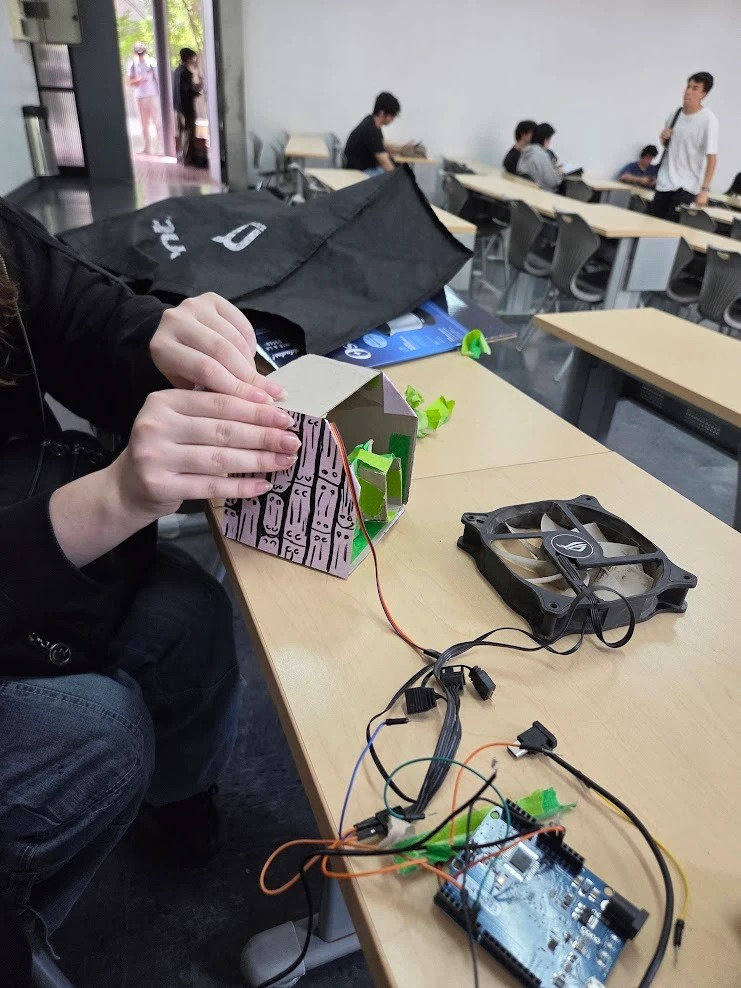
\includegraphics[height=9cm]{v3_foto1.jpg}
			\captionof{figure}{V3: la casa del proyecto, con el ventilador y el Arduino sobre la mesa.}
			\label{fig:v3-foto1}
		\end{center}

		\vspace{0.15cm}
		\noindent\textbf{Qué cambió:}
		% máx. 8 líneas.
		\begin{itemize}
			\item Se mejora el mecanismo del techo de la maqueta para que su movimiento con el viento se note más.
		\end{itemize}
		\pendiente{completar cambios de V3 (máx. 8 líneas)}

		\vspace{0.15cm}
		\noindent\textbf{Por qué cambió — el rationale:}
		% máx. 12 líneas.
		El cambio del techo responde al feedback de la revisión entre pares (R2): el grupo evaluador propuso que el tejado captara mejor el viento. Mejorar su mecanismo hace que el movimiento provocado por el ventilador se note más.
		\pendiente{completar rationale de V3 si hay más (máx. 12 líneas)}

		\vspace{0.15cm}
		\noindent\textbf{Qué se descartó:}
		% máx. 5 líneas.
		Las aletas de papel a los lados de la fachada propuestas en R2: no se alcanzaron a hacer por falta de tiempo y, en V4, se reemplazaron por una palmera.
	\end{versionbox}

	\vspace{0.4cm}

	% ==============================================================================
	% 8. R3 — REVISIÓN CON EL EQUIPO DOCENTE (entre V3 y V4). Máx. 10 líneas.
	% ==============================================================================
	\begin{revisionbox}{R3 — Revisión con el Equipo Docente}{17 de noviembre de 2026}
		\noindent\textbf{Fecha:} 17 de noviembre de 2026.\\
		\textbf{Síntesis de lo discutido:} \pendiente{síntesis}

		\vspace{0.15cm}
		\noindent\textbf{Decisiones tomadas (adoptado / descartado y por qué):}
		\pendiente{decisiones}
	\end{revisionbox}

	\vspace{0.4cm}

	% ==============================================================================
	% 9. V4 — LA EXPERIENCIA FINAL (tras R3)
	%    Experiencia completa y operativa (física, digital y sonora) + balance de cierre.
	%    Si hubo versiones intermedias (V2.5, etc.), van en su lugar cronológico.
	% ==============================================================================
	% FECHA V4: se entrega el jueves 26 de noviembre; actualizar si corresponde.
	\begin{versionbox}{V4 — La Experiencia Final}{24 de noviembre de 2026 · Commits \texttt{fe0400b}, \texttt{58e55ca}}
		\noindent\textbf{Evidencia:}
		\pendiente{fotos y video de V4}
		% VIDEO: \href{https://youtu.be/XXXXXXXXXXX}{https://youtu.be/XXXXXXXXXXX}

		% FOTO: estado físico de V4 (prototipo final, con base y decoración). Aún no hay foto:
		%       guardarla como figuras/v4_foto1.jpg y descomentar.
		% \begin{center}
		% 	\includegraphics[height=9cm]{v4_foto1.jpg}
		% 	\captionof{figure}{V4: prototipo final con base y decoración.}
		% 	\label{fig:v4-foto1}
		% \end{center}

		\vspace{0.15cm}
		\noindent\textbf{Qué cambió:}
		% máx. 8 líneas.
		\begin{itemize}
			\item Versión final: se agrega una base y decoración, que incluye una palmera.
			\item Los botones \textit{Reproducir} y \textit{Activar sonido} se agrandan, llevan ícono (reproducir/pausa y nota musical) y pulsan con más fuerza para llamar la atención. El botón de silencio tiene el mismo tamaño: muestra \textit{Silenciar} y, al silenciar, vuelve a \textit{Activar sonido}.
			\item Al abrir la página aparecen pop-ups de ayuda que indican que se puede hacer clic en cada huracán y en los botones \textit{Reproducir} y \textit{Activar sonido}.
		\end{itemize}
		\pendiente{completar cambios de V4, si hay más (máx. 8 líneas)}

		\vspace{0.15cm}
		\noindent\textbf{Por qué cambió — el rationale:}
		% máx. 12 líneas.
		La palmera responde al feedback de la revisión entre pares (R2): en lugar de las aletas de papel propuestas, que no alcanzamos a hacer por falta de tiempo, se agregó a la maqueta.
		Los botones más grandes y los pop-ups de ayuda salen de la evaluación con usuarios: ambos pensadores evitaron el reproductor, uno dudó antes de tocarlo y la heurística que falló fue que la interacción del reproductor era difícil de descubrir. De esas sesiones salieron como cambios concretos «reproductor más grande y pop-ups» y especificar que se puede hacer clic en el menú.
		\pendiente{completar rationale de V4 si hay más (máx. 12 líneas)}

		\vspace{0.15cm}
		\noindent\textbf{Qué se descartó:}
		% máx. 5 líneas.
		\pendiente{descartes de V4 (máx. 5 líneas)}

		\vspace{0.15cm}
		\noindent\textbf{Balance de cierre:}
		\begin{itemize}
			\item \textbf{Qué mejoró desde V1:} \pendiente{balance}
			\item \textbf{Qué deliberadamente no se cambió y por qué:} \pendiente{balance}
		\end{itemize}
	\end{versionbox}

	\vspace{0.4cm}

	% ==============================================================================
	% 10. EL FEEDBACK AL OTRO GRUPO (§5, en R2) — vale 10 %
	%     Se evalúa la calidad: específico, anclado en principios, constructivo.
	% ==============================================================================
	\section{El Feedback al Otro Grupo}

	\subsection{El Proyecto Evaluado}
	% máx. 5 líneas.
	Proyecto del grupo 8. Visualiza el avance del uso de internet en el mundo a lo largo de los años. Lo físico es a la vez una interacción tangible y una representación del avance de los años: al rotar una caja, la pantalla responde mostrando los datos como puntos sobre un mapa, y el sonido los codifica en su frecuencia.

	\subsection{El Feedback que Dimos}
	% máx. 12 líneas.
	\begin{itemize}
		\item \textbf{Mensaje:} entendimos el uso de internet a lo largo de los años en el mundo.
		\item \textbf{Lo físico:} es una interacción tangible y una representación del avance de los años; aporta a la comprensión y a la retención del usuario.
		\item \textbf{Uso:} rotamos la caja y vimos la respuesta en la pantalla; fue bastante intuitivo.
		\item \textbf{Conservar:} la interacción física, el sonido y los puntos en el mapa, porque son fáciles de interpretar como datos.
		\item \textbf{Cambio 1 (heurística «falta contexto»):} mostrar el avance de los años en la pantalla de forma más visible, más centrado o justo arriba del mapa.
		\item \textbf{Cambio 2 (heurística «la interacción física no es descubrible»):} en la pieza física, indicar visualmente hacia qué lado avanzan los años y que lo que se mueve son años.
	\end{itemize}

	\subsection{Lo que nos Llevamos para Nuestro Proyecto}
	% máx. 5 líneas.
	\pendiente{lo que nos llevamos (máx. 5 líneas)}

	\vspace{0.4cm}

	% ==============================================================================
	% 11. EVALUACIÓN CON USUARIOS — HOJA DEL OBSERVADOR (§8) — vale 10 %
	%     Al menos una ronda de thinking-aloud (idealmente entre V3 y V4), con personas
	%     interactuando físicamente con el prototipo. Pensador externo al grupo que nunca
	%     vio el prototipo; el grupo no interviene ni explica.
	%     Una subsección por ronda: duplicar el bloque "Ronda 1" si hubo más.
	% ==============================================================================
	\section{Evaluación con Usuarios}

	% Transcripción de las dos hojas del observador (Notes_261124_221331.pdf).

	\subsection{Ronda 1}

	\subsubsection{El Pensador}
	% máx. 2 líneas: quién y cuándo (sobre qué versión).
	La madre de Florencia Taís Rojas (integrante del grupo), que nunca había visto el prototipo. Sesión del 24 de noviembre de 2026, sobre la V3.

	\subsubsection{Las Manos También Hablan}
	\begin{itemize}
		\item \textbf{Qué tocó primero:} el recorrido del huracán.
		\item \textbf{Sobre qué dudó antes de tocar:} el menú de huracanes (presionar un botón).
		\item \textbf{Qué zona evitó:} el reproductor y los gráficos.
	\end{itemize}

	\subsubsection{El Sonido, Pensado en Voz Alta}
	\begin{itemize}
		\item \textbf{Qué dato cree que representan los sonidos:} el punto más alto de intensidad, la intensidad y el tocatierra.
		\item \textbf{¿Lo guía o lo confunde?} Le sirve de guía.
	\end{itemize}

	\subsubsection{Bitácora}
	\begin{center}
		\small
		\begin{tabularx}{\textwidth}{lp{6.8cm}X}
			\toprule
			\textbf{Tiempo} & \textbf{Lo que dice (cita literal)} & \textbf{Lo que hace} \\
			\midrule
			0:05 & --- & Lee el título. \\
			0:10 & --- & Lee las muertes. \\
			0:20 & --- & Lee las categorías y el recorrido del mapa con datos. \\
			0:30 & «Hubo más muerte porque hay más gente» & --- \\
			0:50 & --- & Compara las muertes entre huracanes. \\
			1:10 & «No puedo comparar los huracanes» & Ve el recorrido del huracán y lo sigue con el mouse. \\
			--- & «El sonido es porque llega al continente» & --- \\
			1:30 & «Color según categoría» & --- \\
			\bottomrule
		\end{tabularx}
	\end{center}

	\subsubsection{Heurísticas que Fallaron (Zuk-Carpendale)}
	\begin{itemize}
		\item \textbf{Saturación de elementos.}
		\item \textbf{El sonido no se entiende sin explicación:} el sonido se confunde.
	\end{itemize}

	\subsubsection{Las Tres Preguntas de Cierre}
	\begin{enumerate}
		\item \textbf{¿Dónde se atascó más tiempo?} No tocó el menú; hizo clic en el reproductor.
		\item \textbf{¿Qué hipótesis dijo en voz alta que resultó equivocada?} Que el sonido de las muertes era el de la llegada al continente.
		\item \textbf{¿Qué cambio concreto sale de esta sesión?} Aumento horizontal del reproductor y especificar que se puede hacer clic en el menú.
	\end{enumerate}

	\subsubsection{Efecto en el Proceso}
	% Qué transición de versión refleja lo aprendido, o por qué ninguna.
	Se refleja en la transición de V3 a V4: los pop-ups de ayuda indican que se puede hacer clic en cada huracán del menú y en el reproductor, y los botones de reproducir y sonido se agrandaron.

	\subsection{Ronda 2}

	\subsubsection{El Pensador}
	% máx. 2 líneas: quién y cuándo (sobre qué versión).
	El padre de Florencia Taís Rojas (integrante del grupo), que nunca había visto el prototipo. Sesión del 24 de noviembre de 2026, sobre la V3.

	\subsubsection{Las Manos También Hablan}
	\begin{itemize}
		\item \textbf{Qué tocó primero:} el huracán Ida en el menú de huracanes.
		\item \textbf{Sobre qué dudó antes de tocar:} el reproductor.
		\item \textbf{Qué zona evitó:} el reproductor.
	\end{itemize}

	\subsubsection{El Sonido, Pensado en Voz Alta}
	\begin{itemize}
		\item \textbf{Qué dato cree que representan los sonidos:} el gráfico de viento y presión, y la llegada al continente, que coincide con las muertes.
		\item \textbf{¿Lo guía o lo confunde?} Lo mismo \pendiente{¿que le sirve de guía, como al pensador 1?}
	\end{itemize}

	\subsubsection{Bitácora}
	\begin{center}
		\small
		\begin{tabularx}{\textwidth}{lp{6.8cm}X}
			\toprule
			\textbf{Tiempo} & \textbf{Lo que dice (cita literal)} & \textbf{Lo que hace} \\
			\midrule
			--- & «Funciona como menú y los puedo cambiar» & Toca los huracanes del menú. \\
			0:05 & «Este es el recorrido del huracán» & Pasa el mouse por encima de la trayectoria y lee los datos. \\
			--- & --- & Lee los gráficos. \\
			--- & --- & Interpreta los gráficos. \\
			0:15 & --- & Hace scroll. \\
			--- & --- & Interpreta el gráfico de muertes con respecto al recorrido en el mapa. \\
			0:30 & «Acá hay muertes porque llegó al continente» & --- \\
			--- & «Está por orden de fechas» & Vuelve al menú. \\
			1:00 & «Está por orden de impacto, de muertes» & --- \\
			\bottomrule
		\end{tabularx}
	\end{center}

	\subsubsection{Heurísticas que Fallaron (Zuk-Carpendale)}
	\begin{itemize}
		\item \textbf{La interacción no es descubrible:} la interacción del reproductor es difícil de descubrir.
	\end{itemize}

	\subsubsection{Las Tres Preguntas de Cierre}
	\begin{enumerate}
		\item \textbf{¿Dónde se atascó más tiempo?} En la interpretación de los gráficos y en entender el orden del menú.
		\item \textbf{¿Qué hipótesis dijo en voz alta que resultó equivocada?} Que el orden del menú era según las fechas.
		\item \textbf{¿Qué cambio concreto sale de esta sesión?} Un reproductor más grande y pop-ups.
	\end{enumerate}

	\subsubsection{Efecto en el Proceso}
	% Qué transición de versión refleja lo aprendido, o por qué ninguna.
	Se refleja en la transición de V3 a V4: los botones de reproducir y sonido se agrandaron y se agregaron pop-ups de ayuda al abrir la página.

	% ==============================================================================
	% ANEXO — CHECKLIST PREVIO A LA ENTREGA (§12)
	%   Marcar cada ítem cambiando $\square$ por \checkmark solo cuando esté verificado.
	% ==============================================================================
	\vspace{0.4cm}
	\section*{Anexo: Checklist de la Entrega}
	\addcontentsline{toc}{section}{Anexo: Checklist de la Entrega}

	\begin{metabox}
		\begin{itemize}[leftmargin=1.6em]
			\item[$\square$] \textbf{Fisicalización o interacción tangible} presente, en una combinación físico-digital real.
			\item[$\square$] \textbf{La capa digital enriquece} la experiencia; no es decorativa.
			\item[$\square$] \textbf{Sonificación} acorde al contexto físico, con parámetros efectivos (tono, ritmo, timbre) y no solo volumen.
			\item[$\square$] \textbf{Materiales baratos y accesibles}; lo que superó 1000--2000 CLP fue conversado antes con el profesor.
			\item[$\square$] \textbf{Ejemplos revisados}: los del curso y los de Protobject.
			\item[$\square$] \textbf{Revisiones asistidas} con el prototipo y preguntas concretas.
			\item[$\square$] \textbf{Feedback específico} y basado en principios entregado al otro grupo, con su sección en este documento.
			\item[$\square$] \textbf{Evidencia por versión}: fotos, video con interacción y sonido, y commits.
			\item[$\square$] \textbf{El video final} muestra la experiencia completa.
		\end{itemize}
	\end{metabox}

\end{document}
